\iffalse
\let\negmedspace\undefined
\let\negthickspace\undefined
\documentclass[journal,12pt,twocolumn]{IEEEtran}
\usepackage{cite}
\usepackage{amsmath,amssymb,amsfonts,amsthm}
\usepackage{algorithmic}
\usepackage{graphicx}
\usepackage{textcomp}
\usepackage{xcolor}
\usepackage{txfonts}
\usepackage{listings}
\usepackage{enumitem}
\usepackage{mathtools}
\usepackage{gensymb}
\usepackage{comment}
\usepackage[breaklinks=true]{hyperref}
\usepackage{tkz-euclide}
\usepackage{listings}
\usepackage{gvv}
\def\inputGnumericTable{}
\usepackage[latin1]{inputenc}
\usepackage{color}
\usepackage{array}
\usepackage{longtable}
\usepackage{calc}
\usepackage{multirow}
\usepackage{hhline}
\usepackage{ifthen}
\usepackage{lscape}

\newtheorem{theorem}{Theorem}[section]
\newtheorem{problem}{Problem}
\newtheorem{proposition}{Proposition}[section]
\newtheorem{lemma}{Lemma}[section]
\newtheorem{corollary}[theorem]{Corollary}
\newtheorem{example}{Example}[section]
\newtheorem{definition}[problem]{Definition}
\newcommand{\BEQA}{\begin{eqnarray}}
\newcommand{\EEQA}{\end{eqnarray}}
\newcommand{\define}{\stackrel{\triangle}{=}}
\theoremstyle{remark}
\newtheorem{rem}{Remark}
\begin{document}

\bibliographystyle{IEEEtran}
\vspace{3cm}

\title{GATE 2021 BM 46}
\author{EE23BTECH11007 - Aneesh Kadiyala$^{*}$% <-this % stops a space
}
\maketitle
\newpage
\bigskip

\renewcommand{\thefigure}{\theenumi}
\renewcommand{\thetable}{\theenumi}

\vspace{3cm}
\textbf{Question:} Consider a unity feedback system with closed loop transfer function
\begin{align*}
\frac{C\brak{s}}{R\brak{s}} &= \frac{s + 90}{s^2 + 10s + 90}
\end{align*}
The steady state error with respect to a unit ramp input is \rule{1cm}{0.15mm} . \brak{\text{rounded off to one decimal}}

\hfill(GATE 2021 BM)
\\
\solution
\\
\fi
\begin{figure}[h!]
\centering
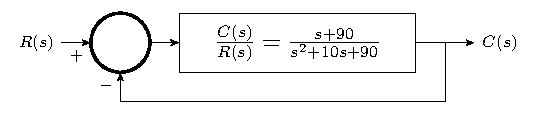
\includegraphics[width=\columnwidth]{2021/BM/46/figs/block-diagram.pdf}
\caption{Block Diagram of the System}
\label{fig:2021bm46-1}
\end{figure}

\begin{align}
\frac{C\brak{s}}{R\brak{s}} &= \frac{s + 90}{s^2 + 10s + 90}
\end{align}
where $C\brak{s}$ is the output and $R\brak{s}$ is the input.
Given that input is unit ramp function:
\begin{align}
r\brak{t} &= tu\brak{t} \\
\implies R\brak{s} &= \frac{1}{s^2} \\
\implies C\brak{s} &= \frac{s + 90}{s^2\brak{s^2+10s+90}} \\
E\brak{s} &= R\brak{s} - C\brak{s} \\
&= \frac{s^2+9s}{s^2\brak{s^2+10s+90}}
\end{align}
Steady state error is:
\begin{align}
\lim_{s\to0}{sE\brak{s}} &= \frac{s + 9}{s^2 + 10s + 90} \\
&= \frac{1}{10}
\end{align}
$\therefore$ steady state error for unit ramp input is 0.1.
\begin{figure}[h!]
\centering
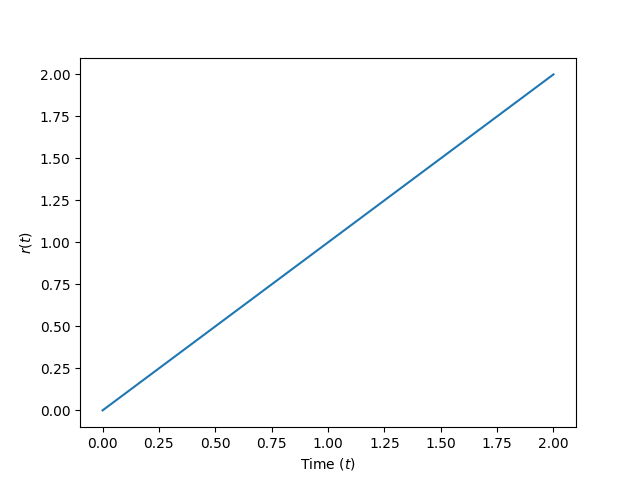
\includegraphics[width=\columnwidth]{2021/BM/46/figs/r_t.png}
\caption{Plot of $r\brak{t}$ vs $t$}
\label{fig:2021bm46-2}
\end{figure}
\begin{align}
C\brak{s} &= \frac{s + 90}{s^2\brak{s^2+10s+90}} \\
&= -\frac{1}{10s} + \frac{1}{s^2} + \frac{s}{10\brak{s^2 + 10s + 90}} \\
&= -\frac{1}{10s} + \frac{1}{s^2} + \frac{s + 5}{\brak{s+5}^2+65} - \frac{1}{2}\brak{\frac{1}{\brak{s+5}^2+65}}
\end{align}
\begin{align}
c\brak{t} &= u\brak{t}\brak{-\frac{1}{10} + t + \frac{e^{-5t}}{10} \cos{\brak{\sqrt{65}t}} - \frac{e^{-5t}}{2\sqrt{65}}\sin{\brak{\sqrt{65}t}}}
\end{align}
\begin{figure}[h!]
\centering
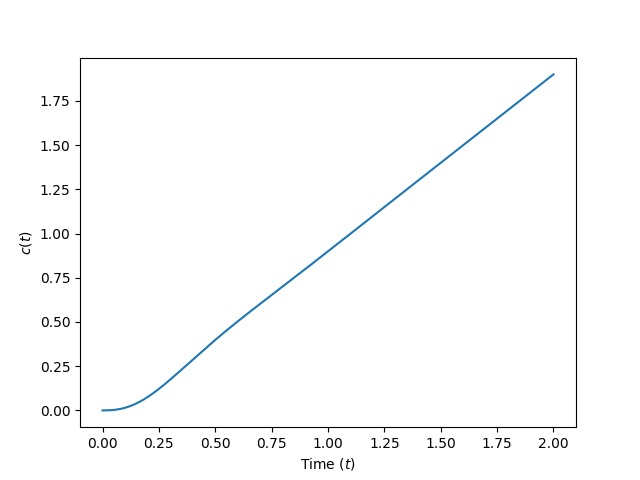
\includegraphics[width=\columnwidth]{2021/BM/46/figs/c_t.png}
\caption{Plot of $c\brak{t}$ vs $t$}
\label{fig:2021bm46-3}
\end{figure}
\begin{align}
E\brak{s} &= R\brak{s} - C\brak{s} \\
\implies e\brak{t} &= r\brak{t} - c\brak{t} \\
&= u\brak{t}\brak{\frac{1}{10} - \frac{e^{-5t}}{10} \cos{\brak{\sqrt{65}t}} + \frac{e^{-5t}}{2\sqrt{65}}\sin{\brak{\sqrt{65}t}}}
\end{align}
\begin{figure}[h!]
\centering
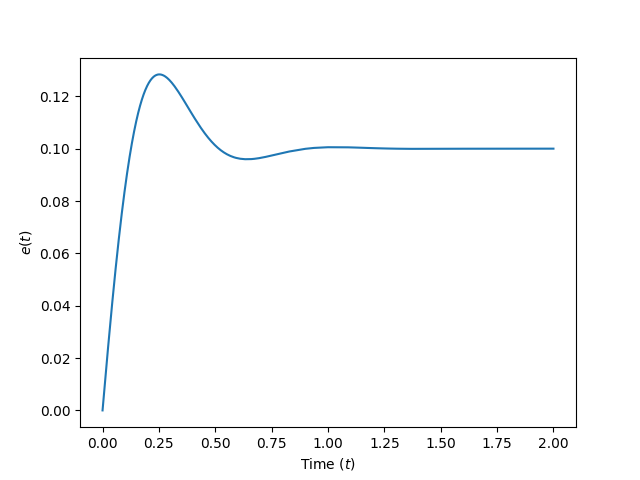
\includegraphics[width=\columnwidth]{2021/BM/46/figs/e_t.png}
\caption{Plot of $e\brak{t}$ vs $t$}
\label{fig:2021bm46-4}
\end{figure}
\begin{align}
\text{Feedback Gain } &= \frac{\frac{C\brak{s}}{R\brak{s}}}{1 + \frac{C\brak{s}}{R\brak{s}}} \\
&= \frac{s + 90}{s^2 + 11s + 180}
\end{align}